\documentclass[12pt]{article}
\usepackage[utf8]{inputenc}
\usepackage[T1]{fontenc}
\usepackage[english]{babel}
\usepackage{floatpag}				% Different pagestyles
\usepackage{amsmath}
\usepackage{array}	
\usepackage{booktabs}
\usepackage{amssymb}
\usepackage{graphicx}
\usepackage{epstopdf}
\usepackage{tabularx}
\usepackage{float}
\usepackage{caption}
\usepackage{subcaption}
\usepackage{parskip}
\usepackage{multirow}
\usepackage{hyperref}
\usepackage{listings}


\begin{document}

\title{Project1}


\section*{Introduction}

This report is going to look in to matrix handling using different approaches. 
Comparing LU decomposition and tridiagonal decomposition approach. An attempt on c++ programming is done to look at the differences in methods in run time and accuracy. 



\section*{Theory}


Poisson's equation: 

\begin{equation}
 \nabla^2 \Phi = -4\pi \rho(r)
\end{equation}


Which becomes in one dimension with symmetric $\Phi$ 

\begin{equation}
\frac{1}{r^2} \frac{d}{dr}(r^2\frac{d\Phi}{dr}) = -4\pi \rho(r)
\end{equation}


Starting by looking at the relation 
$\textbf{Av} = \tilde{\textbf{b}}$

Where \textbf{A} =
$$
\begin{bmatrix}
2 & -1 & 0 & \ldots & \ldots & 0 \\
-1 & 2 & -1 & 0 &\ldots & \vdots \\ 
0 & -1 & 2 & -1 & 0 & \vdots \\
\vdots & \vdots & \ddots & \ddots & \ddots & \vdots\\ 
\vdots & \ldots & \ldots & -1 & 2 & -1\\
0 & \ldots & \ldots & 0 & -1 & 2\\
\end{bmatrix}
$$

and \textbf{v} = $$\begin{bmatrix}
v_1\\
v_2\\
v_3\\
\ldots\\
v_{n-1}\\
v_{n}\\
\end{bmatrix}
$$

\begin{equation}
f_i = -\frac{v_{i+1} +v_{i-1} -2v_i}{h^2}
\label{eq1}
\end{equation}

From \ref{eq1} can be rewritten as a linear equation \textbf{Av} = \textbf{b} where $\textbf{b} = h^2\textbf{f}$. This by 

$\textbf{b} = -h^2*\frac{v_{i+1} +v_{i-1} -2v_i}{h^2}$

$\textbf{b} = a*v_{i+1} + b*v_i + c*v_{i-1}$

Where a = c = -1 and b = 2.

Which equals $A(i)*v(i)$.

The function $f(i) = e^{-10x}$.

The relative error is given by 

\begin{equation}
\epsilon_i = \log_{10}(|\frac{v_i - u_i}{u_i}|)
\label{eq:rel}
\end{equation}

Computation start with a forward substitution the a backward substitution to get the approximation of the value v in the equation $\textbf{Av} = \textbf{b}$.  The important bit of code that gives the first method:  
 
\begin{lstlisting}
{double btemp = b(0);
u(1) = f(0)/btemp;
for(i=1 ; i < n ; i++) {
    temp(i) = c(i-1)/btemp;
    btemp = b(i)-a(i)*temp(i);
    u(i) = (f(i) - a(i)*u(i-1)/btemp);
    }

//cout<<u<<endl;
//backward substitution loop
for(i=n-2; i>=0; i--){
    u(i) -= temp(i+1)*u(i+1);
}}
\end{lstlisting} 




Codes: 

plot.py , main.cpp

Found in Project1/project1 at \url{https://github.com/magnusji/compfys.git}


\section*{Results}

\begin{table}[hb!]
\centering
\caption{Run time for each method}
\begin{tabular}{c|c|c|}
N & Tri & LU \\
\hline
10 & 5.5e-05 & 0.000175 \\
100 & 0.000151 & 0.000858 \\
1000 & 0.00101 & 0.07432\\

\end{tabular}
\label{tab:time}
\end{table}

The Table \ref{tab:time} shows the difference in runtime between the two methods. 
And Figure \ref{fig:app} shows how the methods compare against closed form solution. 


\begin{figure}[hb!]
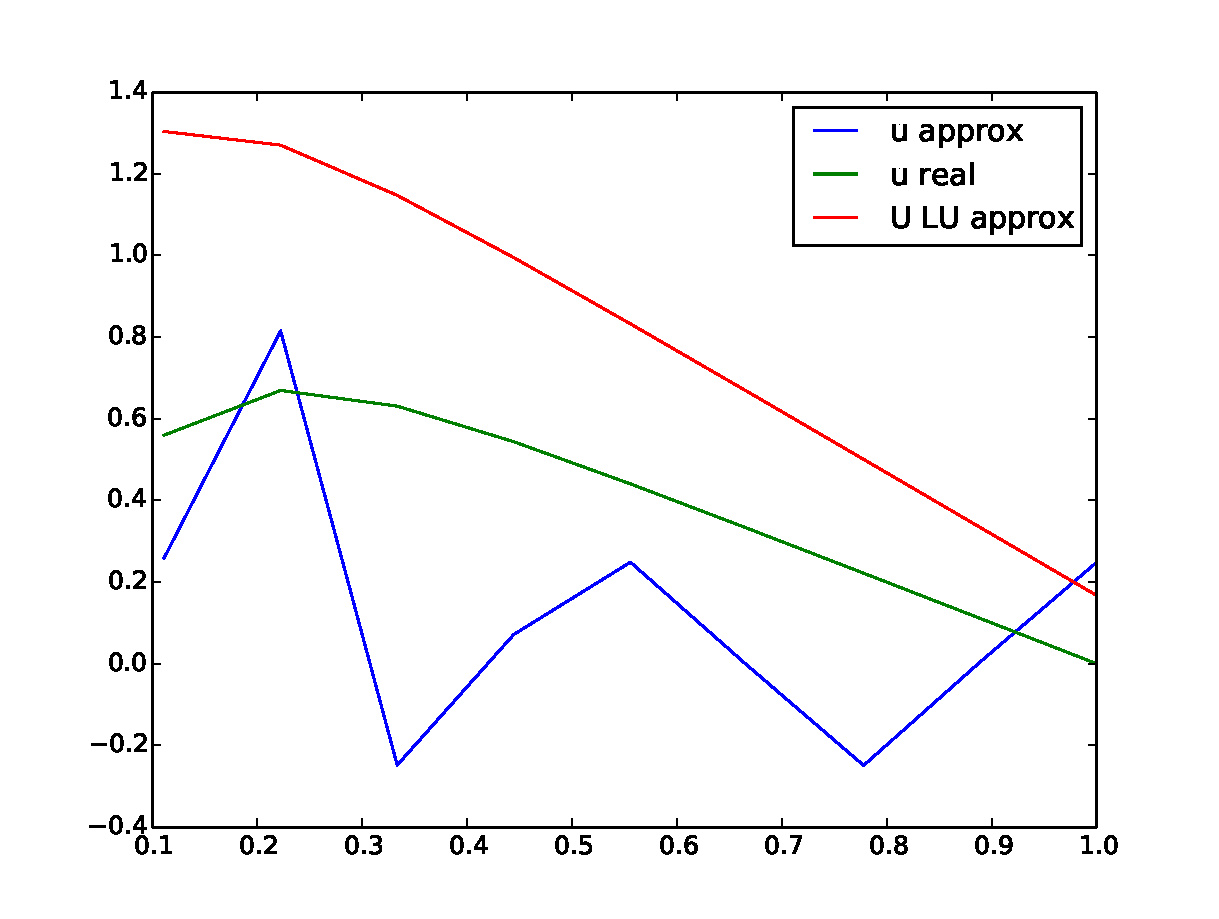
\includegraphics[width=\textwidth]{./results/figure_10pt.pdf}
\caption{Approximations for Tridiagonal system and LU decomposition and the exact soulution}
\label{fig:app}
\end{figure}

The relative error is given by Equation \ref{eq:rel}
and shows  $epsu = inf epsv = inf$. 

More results in \url{https://github.com/magnusji/compfys.git}. 

\section*{Discussion}

The run time for the first method is always better than for LU decomposition. And also didn't have that much problems with larger matrices. The LU decomposition couldn't go further than size 1000X1000 matrix.

But from Figure \ref{fig:app} it seems like the LU decomposition method follows the curve better than the first method. But since the relative error maximum only shows inf it is hard to say which is more accurate. 

There is much in the programs that should be improved. Both the relative error should be improved so that it is working, the max error is larger than it looks like in the printed file. Also the plot should be done by reading from file instead of what is done here by copying values. So much to be improved.  





\end{document}